\documentclass{article}
\usepackage{tikz}
\usetikzlibrary{arrows.meta,positioning,calc,shapes.geometric}
\pagestyle{empty}
\begin{document}
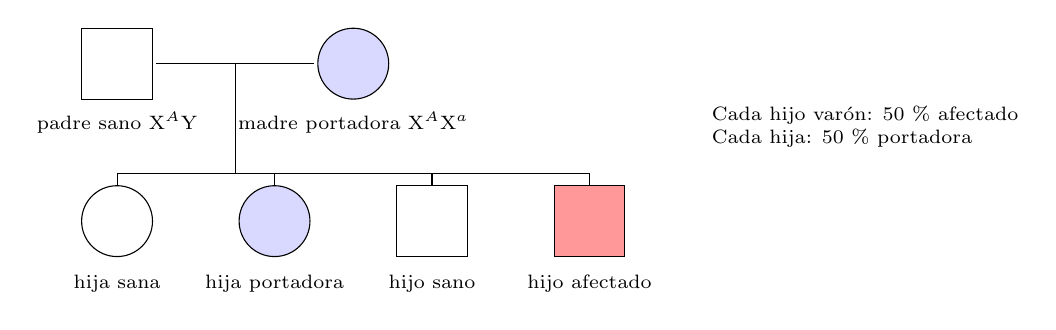
\begin{tikzpicture}
\tikzset{every node/.append style={align=center}}

\def\sq#1#2#3{\node[draw, fill=#3, minimum size=0.9cm] at (#1,#2) {};}
\def\ci#1#2#3{\node[draw, circle, fill=#3, minimum size=0.9cm] at (#1,#2) {};}
\sq{0}{3.2}{white}\node[font=\scriptsize] at (0,2.45) {padre sano X$^A$Y}; \ci{3.0}{3.2}{blue!15}\node[font=\scriptsize] at (3.0,2.45) {madre portadora X$^A$X$^a$};
\draw (0.5,3.2) -- (2.5,3.2); \draw (1.5,3.2) -- (1.5,1.8);
\ci{0}{1.2}{white}\ci{2.0}{1.2}{blue!15}\sq{4.0}{1.2}{white}\sq{6.0}{1.2}{red!40}
\node[font=\scriptsize, align=center] at (0,0.4) {hija sana}; \node[font=\scriptsize, align=center] at (2.0,0.4) {hija portadora}; \node[font=\scriptsize, align=center] at (4.0,0.4) {hijo sano}; \node[font=\scriptsize, align=center] at (6.0,0.4) {hijo afectado};
\draw (0,1.8) -- (6,1.8); \foreach \x in {0,2,4,6} {\draw (\x,1.8) -- (\x,1.65);}
\node[font=\scriptsize, align=left] at (9.5,2.4) {Cada hijo varón: 50 \% afectado\\ Cada hija: 50 \% portadora};

\end{tikzpicture}
\end{document}
